\documentclass[preprint,12pt]{elsarticle}

\usepackage{graphicx}
\usepackage{booktabs}
\usepackage{adjustbox}
\usepackage{hyperref}
\usepackage[section]{placeins}
\hypersetup{hidelinks}

\journal{Computer Methods and Programs in Biomedicine}
\graphicspath{{figures/}{./}}
\renewcommand{\thefigure}{S\arabic{figure}}
\renewcommand{\thetable}{S\arabic{table}}

\begin{document}

\begin{frontmatter}
\title{Supplementary Material for ``A Reproducible ROI-Robust Evaluation and Mobile Distillation Framework for Ultrasound Lesion Classification''}
\author[inst1]{Zihan Li}
\author[inst1]{Cong Yang}
\affiliation[inst1]{organization={School of Future Science and Engineering, Soochow University},
            city={Suzhou},
            postcode={215222},
            state={Jiangsu},
            country={China}}
\end{frontmatter}

\section{Supplementary Tables}

Table~\ref{tab:s_validation_audit} records the validation-performance audit used to reduce test-set model-selection risk. The selected model is retained for the original dataset-specific benchmark, while the main manuscript also reports the stronger MUDD+DA-noMCA robustness variant evaluated on the frozen analysis-label snapshot.

\begin{table}[!htbp]
    \centering
    \small
    \caption{Validation-performance audit for the TransXNet-family selection. Values are averages over three TN5000 seeds or five BUSI/AUL training folds.}
    \label{tab:s_validation_audit}
    \begin{adjustbox}{max width=\textwidth}
    \begin{tabular}{lccccc}
        \toprule
        Variant & TN5000 val AUC & BUSI val AUC & AUL val AUC & Mean val AUC & Selected \\
        \midrule
        TransXNet & 0.9577 & 0.7796 & 0.7464 & 0.8279 & no \\
        TransXNet-GG & 0.9632 & 0.8011 & 0.7390 & 0.8345 & no \\
        GGG-noMCA & \textbf{0.9700} & 0.8957 & 0.8798 & 0.9152 & no \\
        UL-TransXNet & 0.9638 & \textbf{0.9199} & \textbf{0.8827} & \textbf{0.9222} & yes \\
        \bottomrule
    \end{tabular}
    \end{adjustbox}
\end{table}

The comparison pool uses the same ROI construction, augmentation family, validation-based thresholding, and reporting scripts, but the unusually low ResNet50 TN5000 result remains a baseline-sanity risk. We retain it for transparency rather than using it as the primary comparison point. The main manuscript therefore compares UL-TransXNet with the strongest observed comparison baseline on each dataset, while the release artifacts include the repeated-run logs and prediction files needed to inspect whether ResNet50 instability comes from this ROI protocol, optimization sensitivity, or implementation details.

\begin{table}[!htbp]
    \centering
    \small
    \caption{Complexity--performance trade-off of the comparison pool. CUDA latency is local workstation model-only batch-1 latency. Mean AUC and Mean BalAcc are unweighted averages over TN5000, BUSI, and AUL.}
    \label{tab:s_complexity_table}
    \begin{adjustbox}{max width=\textwidth}
    \begin{tabular}{lccccccccc}
        \toprule
        Method & Input & Params & MACs & CUDA ms & TN5000 & BUSI & AUL & Mean AUC & Mean BalAcc \\
        \midrule
        MobileNetV3-Large & 256 & 4.86M & 0.28G & 3.17 & 0.8282 & 0.7947 & 0.7357 & 0.7862 & 0.7183 \\
        EfficientNet-B0 & 256 & 4.66M & 0.50G & 6.53 & 0.7856 & 0.7659 & 0.6099 & 0.7205 & 0.6682 \\
        EfficientFormer-L1 & 224 & 11.62M & 1.31G & 3.41 & 0.9249 & 0.7917 & 0.7196 & 0.8121 & 0.7330 \\
        RepViT-M1.1 & 256 & 8.04M & 1.80G & 5.19 & 0.8403 & 0.8028 & 0.6797 & 0.7742 & 0.7020 \\
        UL-TransXNet & 256 & 14.37M & 2.36G & 30.23 & \textbf{0.9532} & \textbf{0.8485} & 0.8248 & \textbf{0.8755} & \textbf{0.8037} \\
        DenseNet121 & 256 & 7.48M & 3.70G & 7.19 & 0.9360 & 0.8154 & 0.6729 & 0.8081 & 0.7401 \\
        ResNet50 & 256 & 24.56M & 5.40G & 3.25 & 0.6531 & 0.7519 & 0.5481 & 0.6510 & 0.6190 \\
        ConvNeXt-Tiny & 256 & 28.21M & 5.82G & 3.30 & 0.9508 & 0.8050 & 0.8274 & 0.8611 & 0.7651 \\
        Swin-T & 256 & 27.91M & 7.11G & 6.32 & 0.9497 & 0.8190 & \textbf{0.8319} & 0.8669 & 0.7901 \\
        \bottomrule
    \end{tabular}
    \end{adjustbox}
\end{table}

\begin{table}[!htbp]
    \centering
    \small
    \caption{Two-device Android repeat for the exported teacher and distilled students. Both devices use the paper-log TN5000 analysis-label snapshot, file-mode ROI loading, 30\% expanded non-square crops, and five hot runs per model.}
    \label{tab:s_android_two_device}
    \begin{adjustbox}{max width=\textwidth}
    \begin{tabular}{llcccc}
        \toprule
        Device & Model & Android AUC & Hot total ms & Hot inference ms & P95 total ms \\
        \midrule
        Xiaomi 24129PN74C & EfficientFormer-L1+KD & 0.9634 & 32.690 & 31.298 & 37.667 \\
        Xiaomi 24129PN74C & EfficientFormer-L1+ECA+KD & 0.9576 & 34.853 & 33.390 & 41.103 \\
        Xiaomi 24129PN74C & GGG-MCA teacher & 0.9433 & 130.551 & 128.831 & 132.464 \\
        Samsung SM-X800 & EfficientFormer-L1+KD & 0.9634 & 55.954 & 54.697 & 67.714 \\
        Samsung SM-X800 & EfficientFormer-L1+ECA+KD & 0.9576 & 56.159 & 54.852 & 58.328 \\
        Samsung SM-X800 & GGG-MCA teacher & 0.9433 & 168.450 & 166.806 & 170.529 \\
        \bottomrule
    \end{tabular}
    \end{adjustbox}
\end{table}

\begin{table}[!htbp]
    \centering
    \small
    \caption{Offline paired statistical comparison between UL-TransXNet and the strongest comparison baseline in the main benchmark table after recomputation with the frozen paper-log labels. These are repeated-run stability checks, not large-sample clinical significance tests.}
    \label{tab:s_paired_stats}
    \begin{adjustbox}{max width=\textwidth}
    \begin{tabular}{lllcccc}
        \toprule
        Dataset & Baseline & Metric & n & $\Delta$ & Run-delta range & p \\
        \midrule
        TN5000 & ConvNeXt-Tiny & AUC & 3 & +0.0024 & [-0.0024, +0.0051] & 1.0000 \\
        TN5000 & ConvNeXt-Tiny & BalAcc & 3 & +0.0058 & [-0.0023, +0.0215] & 1.0000 \\
        BUSI & Swin-T & AUC & 5 & +0.0294 & [+0.0179, +0.0422] & 0.0625 \\
        BUSI & Swin-T & BalAcc & 5 & +0.0714 & [+0.0460, +0.0989] & 0.0625 \\
        AUL & Swin-T & AUC & 5 & -0.0071 & [-0.0189, +0.0203] & 0.3750 \\
        AUL & Swin-T & BalAcc & 5 & -0.0376 & [-0.1117, +0.0869] & 0.3750 \\
        \bottomrule
    \end{tabular}
    \end{adjustbox}
\end{table}

\begin{table}[!htbp]
    \centering
    \small
    \caption{Android baseline context on the Xiaomi 24129PN74C device. AUC values use the paper-log TN5000 analysis-label snapshot; latency is the measured hot end-to-end runtime.}
    \label{tab:s_android_baselines}
    \begin{adjustbox}{max width=\textwidth}
    \begin{tabular}{lccc}
        \toprule
        Model & Android AUC & Hot total latency (ms) & Model size (MB) \\
        \midrule
        MobileNetV3-Large & 0.8146 & 15.745 & 18.528 \\
        EfficientFormer-L1 & 0.9168 & 34.451 & 44.303 \\
        RepViT-M1.1 & 0.9035 & 46.188 & 30.749 \\
        ConvNeXt-Tiny & 0.9505 & 169.662 & 107.718 \\
        GGG-MCA teacher & 0.9433 & 130.551 & 53.458 \\
        EfficientFormer-L1+KD & \textbf{0.9634} & \textbf{32.690} & 44.303 \\
        EfficientFormer-L1+ECA+KD & 0.9576 & 34.853 & 44.304 \\
        \bottomrule
    \end{tabular}
    \end{adjustbox}
\end{table}

\begin{table}[!htbp]
    \centering
    \small
    \caption{Closed-loop automatic ROI classification summary. Oracle uses annotation boxes, auto uses detector-derived boxes, and full resizes the whole image.}
    \label{tab:s_auto_roi}
    \begin{adjustbox}{max width=\textwidth}
    \begin{tabular}{llcccc}
        \toprule
        Dataset & Input & AUC & BalAcc & F1 & Acc \\
        \midrule
        BUSI & oracle & 0.8485 & 0.7851 & 0.7695 & 0.7984 \\
        BUSI & auto & 0.8393 & 0.7809 & 0.7667 & 0.7969 \\
        BUSI & full & 0.7575 & 0.7064 & 0.6710 & 0.6961 \\
        AUL & oracle & 0.8248 & 0.7407 & 0.7215 & 0.7323 \\
        AUL & auto & 0.8094 & 0.7358 & 0.7124 & 0.7244 \\
        AUL & full & 0.7104 & 0.6268 & 0.6307 & 0.6866 \\
        \bottomrule
    \end{tabular}
    \end{adjustbox}
\end{table}

\begin{table}[!htbp]
    \centering
    \small
    \caption{Detector localization quality used for automatic ROI construction. TN5000 values are mean $\pm$ standard deviation across three detector seeds on the official test split; BUSI/AUL values are mean $\pm$ standard deviation across five detector folds on the fixed held-out test sets.}
    \label{tab:s_detector_quality}
    \begin{adjustbox}{max width=\textwidth}
    \begin{tabular}{lcccc}
        \toprule
        Dataset & Mean IoU & R@0.50 & R@0.75 & No det. \\
        \midrule
        TN5000 & 0.7855 $\pm$ 0.0033 & 0.9350 $\pm$ 0.0035 & 0.7880 $\pm$ 0.0035 & 0.0000 \\
        BUSI & 0.7365 $\pm$ 0.0241 & 0.8403 $\pm$ 0.0141 & 0.6822 $\pm$ 0.0548 & 0.0000 \\
        AUL & 0.5755 $\pm$ 0.0221 & 0.6740 $\pm$ 0.0419 & 0.4331 $\pm$ 0.0201 & 0.0000 \\
        \bottomrule
    \end{tabular}
    \end{adjustbox}
\end{table}

\begin{table}[!htbp]
    \centering
    \small
    \caption{Descriptive BUSI duplicate and near-duplicate audit. The audit uses the diagnostic labels from the BUSI label manifest, not the one-class detector labels stored in VOC XML files. It does not alter the public-benchmark split or main reported metrics. Near duplicates require both dHash and aHash Hamming distances at or below the stated threshold.}
    \label{tab:s_busi_duplicate_audit}
    \begin{adjustbox}{max width=\textwidth}
    \begin{tabular}{lccccc}
        \toprule
        Hash screen & Exact duplicate pairs & Near-duplicate pairs & Cross-split pairs & Label-conflict pairs & Output directory \\
        \midrule
        Strict ($\leq 2$) & 1 & 88 & 26 & 6 & \texttt{busi\_duplicate\_audit\_20260510\_manifestlabels\_t2} \\
        Relaxed ($\leq 5$) & 1 & 141 & 41 & 9 & \texttt{busi\_duplicate\_audit\_20260510\_manifestlabels\_t5} \\
        \bottomrule
    \end{tabular}
    \end{adjustbox}
\end{table}

\begin{table}[!htbp]
    \centering
    \small
    \caption{Case-level uncertainty and calibration summary for seed/fold-averaged UL-TransXNet predictions recomputed with the frozen paper-log labels. ECE uses 10 confidence bins.}
    \label{tab:s_calibration_uncertainty}
    \begin{adjustbox}{max width=\textwidth}
    \begin{tabular}{lcccc}
        \toprule
        Dataset & AUC 95\% CI & BalAcc 95\% CI & ECE & Brier \\
        \midrule
        TN5000 & 0.960 [0.946, 0.973] & 0.909 [0.892, 0.930] & 0.0226 & 0.0662 \\
        BUSI & 0.850 [0.756, 0.932] & 0.800 [0.746, 0.884] & 0.0538 & 0.1770 \\
        AUL & 0.826 [0.733, 0.903] & 0.832 [0.760, 0.902] & 0.1474 & 0.1979 \\
        \bottomrule
    \end{tabular}
    \end{adjustbox}
\end{table}

\begin{table}[!htbp]
    \centering
    \small
    \caption{Case-level diagnostic statistics for seed/fold-averaged UL-TransXNet predictions on the fixed test sets. Brackets are case-bootstrap 95\% confidence intervals.}
    \label{tab:s_case_level_stats}
    \begin{adjustbox}{max width=\textwidth}
    \begin{tabular}{lcccccc}
        \toprule
        Dataset & AUC & Sens. & Spec. & PPV & NPV & ECE/Brier \\
        \midrule
        TN5000 & 0.960 [0.946, 0.973] & 0.893 & 0.925 & 0.968 & 0.772 & 0.023/0.066 \\
        BUSI & 0.850 [0.756, 0.932] & 0.711 & 0.890 & 0.730 & 0.880 & 0.054/0.177 \\
        AUL & 0.826 [0.733, 0.903] & 0.892 & 0.773 & 0.881 & 0.791 & 0.147/0.198 \\
        \bottomrule
    \end{tabular}
    \end{adjustbox}
\end{table}

\FloatBarrier

\section{Descriptive Complexity Views}

Figure~\ref{fig:s_teaser_tradeoff} keeps the original accuracy--complexity visualization as a descriptive summary. It is not used as the main evidence for model selection because the vertical axis averages dataset-specific test AUC values from datasets with different organs, sizes, and prevalence. The main manuscript therefore uses protocol-separated tables and mobile latency analysis for the primary claims.

\begin{figure}[!htbp]
    \centering
    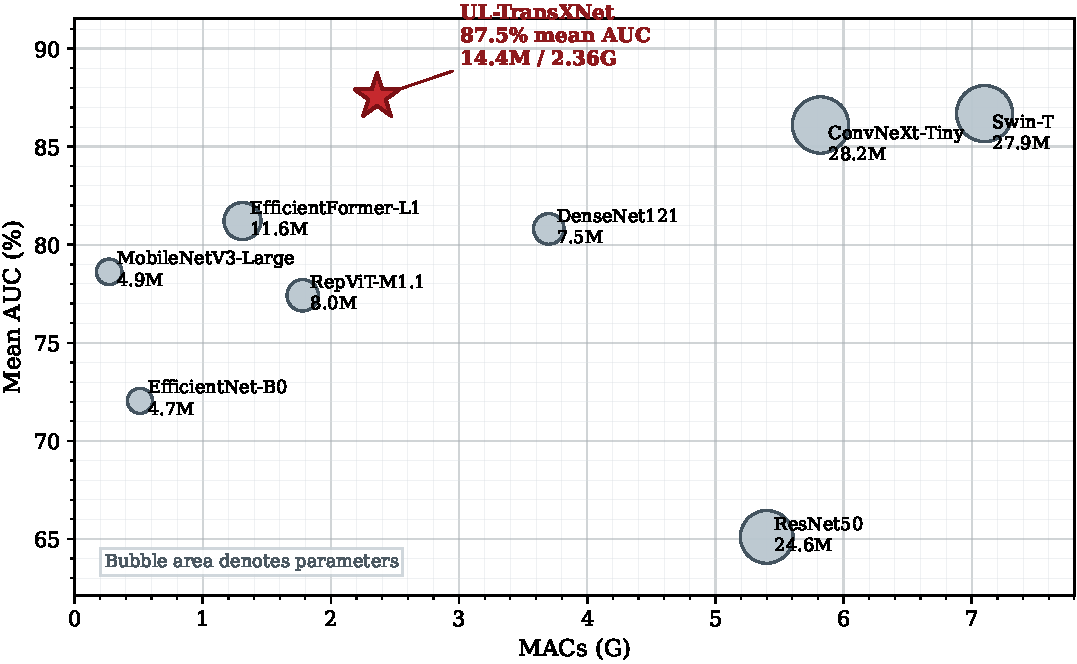
\includegraphics[width=0.95\textwidth]{fig_teaser_tradeoff_crop.pdf}
    \caption{Descriptive mean AUC versus MACs view. Mean AUC is the unweighted average over TN5000, BUSI, and AUL under dataset-specific training; it should not be interpreted as external cross-organ validation.}
    \label{fig:s_teaser_tradeoff}
\end{figure}

\begin{figure}[!htbp]
    \centering
    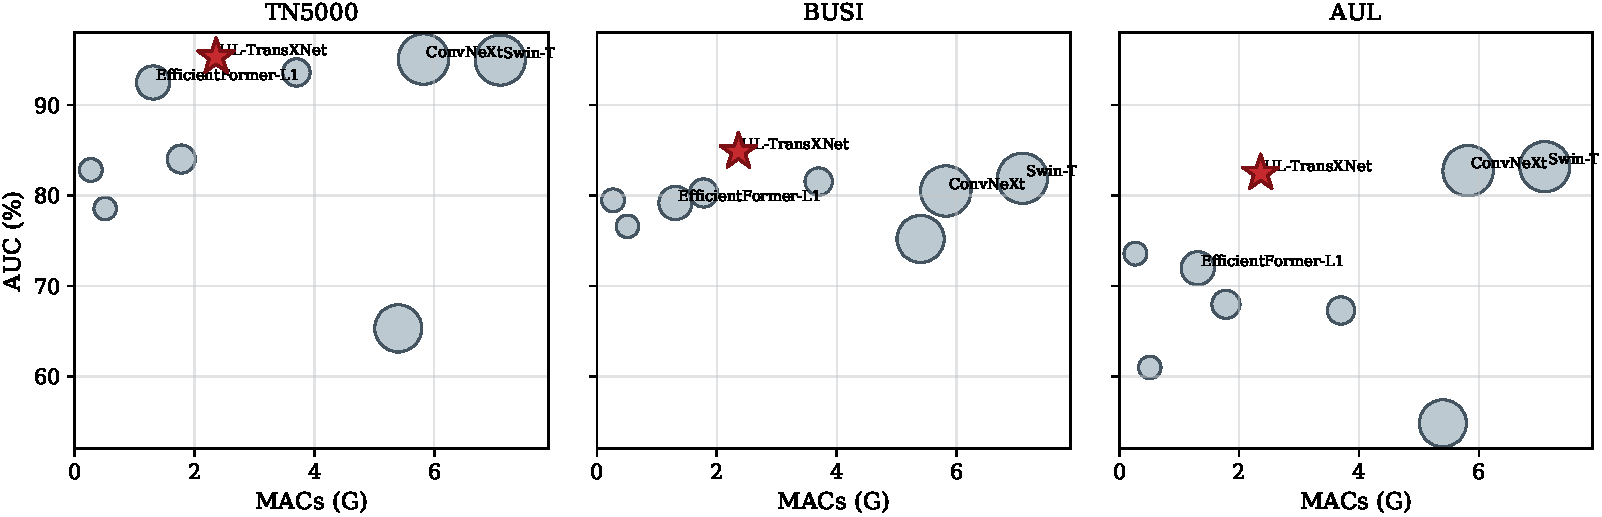
\includegraphics[width=0.95\textwidth]{fig_complexity_tradeoff_auc_crop.pdf}
    \caption{Additional complexity--AUC trade-off visualization from the original benchmark package. This figure is retained for reference but secondary to the protocol-separated result tables.}
    \label{fig:s_complexity_tradeoff}
\end{figure}

\FloatBarrier

\section{Additional Diagnostic Figures}

\begin{figure}[!htbp]
    \centering
    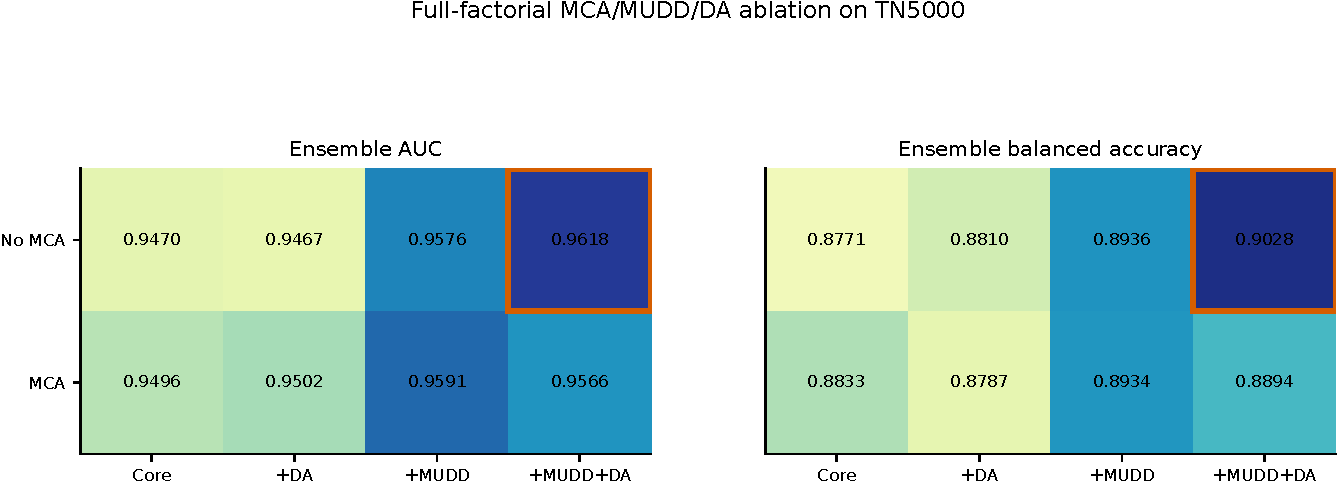
\includegraphics[width=0.85\textwidth]{fig_factorial_ablation_heatmap_crop.pdf}
    \caption{Heatmap view of the full-factorial TN5000 MCA/MUDD/differential-attention ablation. The main manuscript reports the corresponding numerical table.}
    \label{fig:s_factorial_heatmap}
\end{figure}

\begin{figure}[!htbp]
    \centering
    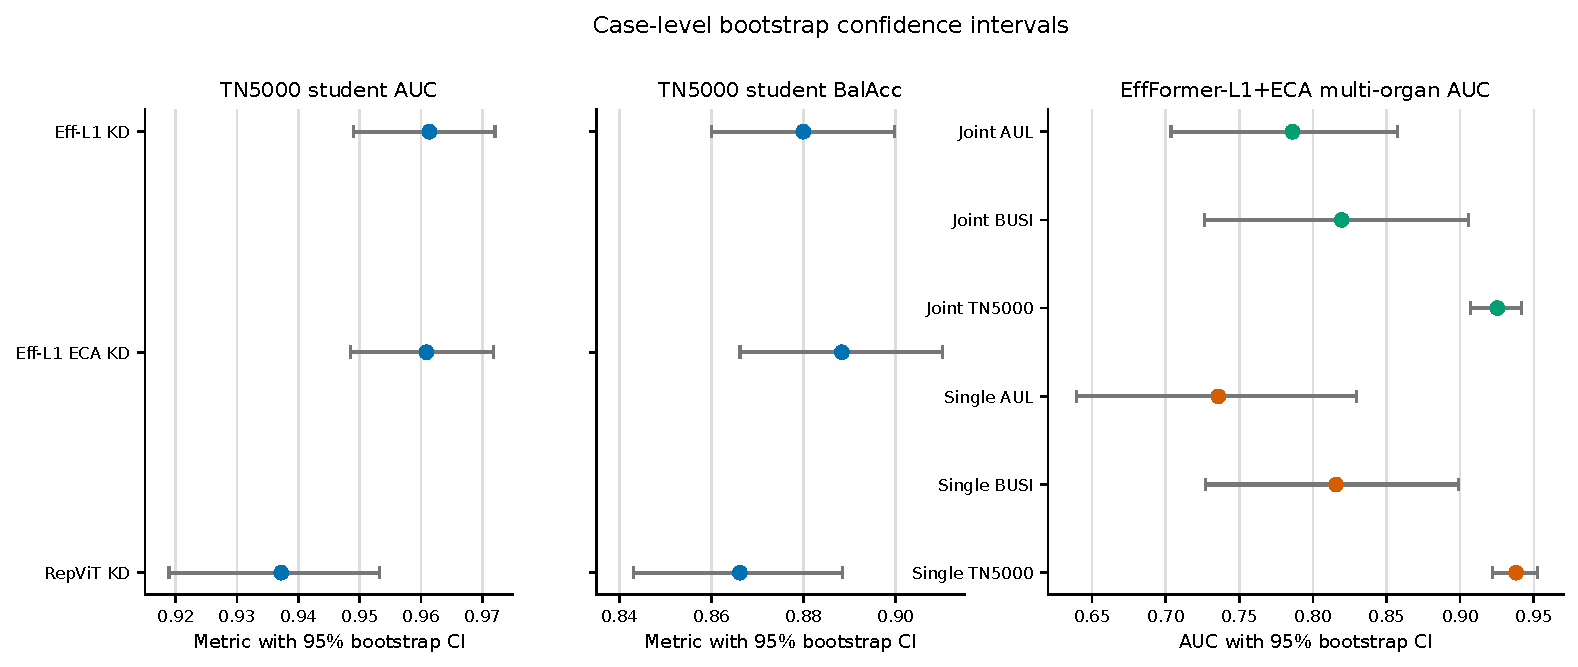
\includegraphics[width=0.85\textwidth]{fig_bootstrap_ci_forest.pdf}
    \caption{Bootstrap confidence-interval forest plot for selected frozen-snapshot experiments. Case-level intervals are provided as statistical transparency rather than clinical significance claims.}
    \label{fig:s_bootstrap_ci}
\end{figure}

\begin{figure}[!htbp]
    \centering
    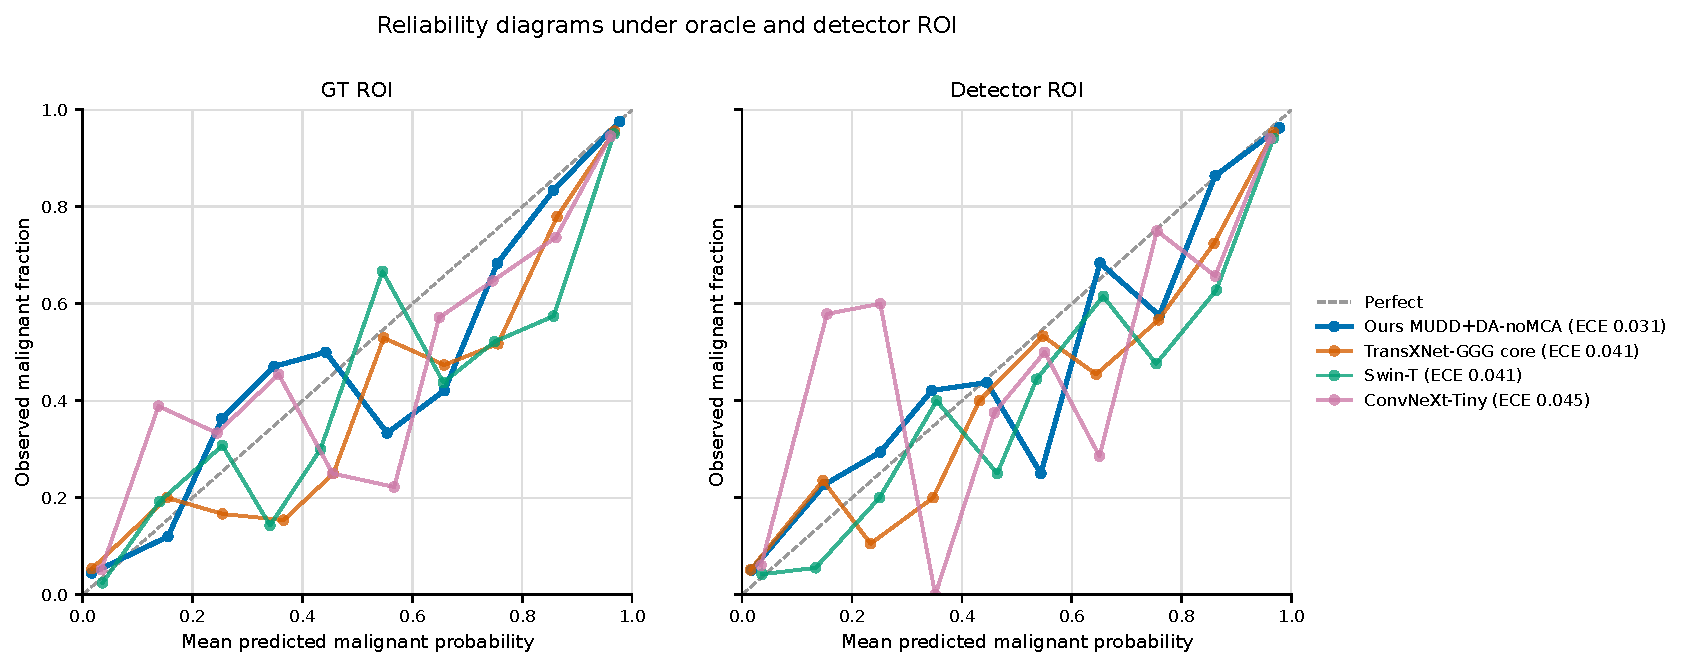
\includegraphics[width=0.85\textwidth]{fig_reliability_oracle_detector.pdf}
    \caption{Reliability and calibration diagnostics for oracle and detector-derived ROI settings. These plots support the manuscript's cautious discussion of probability calibration.}
    \label{fig:s_reliability}
\end{figure}

\begin{figure}[!htbp]
    \centering
    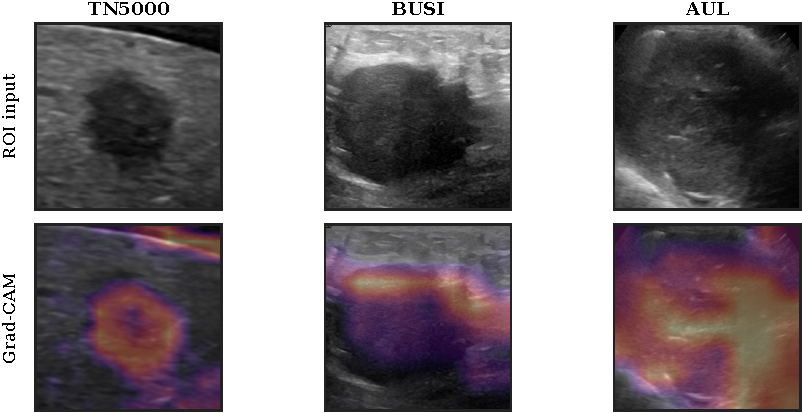
\includegraphics[width=0.85\textwidth]{fig_gradcam_sanity_crop.pdf}
    \caption{Grad-CAM examples used as qualitative sanity checks. They are not interpreted as causal explanations of model decisions.}
    \label{fig:s_gradcam}
\end{figure}

\end{document}
